% Digital Logic Report Template
% Created: 2020-01-10, John Miller

%==========================================================
%=========== Document Setup  ==============================

% Formatting defined by class file
\documentclass[11pt]{article}

% ---- Document formatting ----
\usepackage[margin=1in]{geometry}	% Narrower margins
\usepackage{booktabs}				% Nice formatting of tables
\usepackage{graphicx}				% Ability to include graphics

%\setlength\parindent{0pt}	% Do not indent first line of paragraphs 
\usepackage[parfill]{parskip}		% Line space b/w paragraphs
%	parfill option prevents last line of pgrph from being fully justified

% Parskip package adds too much space around titles, fix with this
\RequirePackage{titlesec}
\titlespacing\section{0pt}{8pt plus 4pt minus 2pt}{3pt plus 2pt minus 2pt}
\titlespacing\subsection{0pt}{4pt plus 4pt minus 2pt}{-2pt plus 2pt minus 2pt}
\titlespacing\subsubsection{0pt}{2pt plus 4pt minus 2pt}{-6pt plus 2pt minus 2pt}

% ---- Hyperlinks ----
\usepackage[colorlinks=true,urlcolor=blue]{hyperref}	% For URL's. Automatically links internal references.

% ---- Code listings ----
\usepackage{listings} 					% Nice code layout and inclusion
\usepackage[usenames,dvipsnames]{xcolor}	% Colors (needs to be defined before using colors)

% Define custom colors for listings
\definecolor{listinggray}{gray}{0.98}		% Listings background color
\definecolor{rulegray}{gray}{0.7}			% Listings rule/frame color

% Style for Verilog
\lstdefinestyle{Verilog}{
	language=Verilog,					% Verilog
	backgroundcolor=\color{listinggray},	% light gray background
	rulecolor=\color{blue}, 			% blue frame lines
	frame=tb,							% lines above & below
	linewidth=\columnwidth, 			% set line width
	basicstyle=\small\ttfamily,	% basic font style that is used for the code	
	breaklines=true, 					% allow breaking across columns/pages
	tabsize=3,							% set tab size
	commentstyle=\color{gray},	% comments in italic 
	stringstyle=\upshape,				% strings are printed in normal font
	showspaces=false,					% don't underscore spaces
}

% How to use: \Verilog[listing_options]{file}
\newcommand{\Verilog}[2][]{%
	\lstinputlisting[style=Verilog,#1]{#2}
}




%======================================================
%=========== Body  ====================================
\begin{document}

\title{ELC 2137 Lab \08: 4-digit Display}
\author{Spencer Stinson}

\maketitle


\section*{Summary}

In this experiment, we used the skills we had learned in the previous two labs to apply it to our 4 digit display. This display was able to show us BCD and hex conversions in one device. This device used many different converters that we had previously made to work together for the final product. 

\section*{Code}

\Verilog[caption= mux2 code]{C:/Users/spencer_stinson1/Documents/GitHub/Lab08/Lab_08/Lab_08.srcs/sources_1/new/mux2.sv}
\Verilog[caption= mux4 code]{C:/Users/spencer_stinson1/Documents/GitHub/Lab08/Lab_08/Lab_08.srcs/sources_1/new/mux4.sv}
\Verilog[caption= an decoder code]{C:/Users/spencer_stinson1/Documents/GitHub/Lab08/Lab_08/Lab_08.srcs/sources_1/new/an_decoder.sv}
\Verilog[caption= sseg4 code]{C:/Users/spencer_stinson1/Documents/GitHub/Lab08/Lab_08/Lab_08.srcs/sources_1/new/sseg4.sv}
\Verilog[caption= sseg4 manual code]{C:/Users/spencer_stinson1/Documents/GitHub/Lab08/Lab_08/Lab_08.srcs/sources_1/new/sseg4_manual.sv}


\section*{Results}
\begin{figure}[ht]\centering 
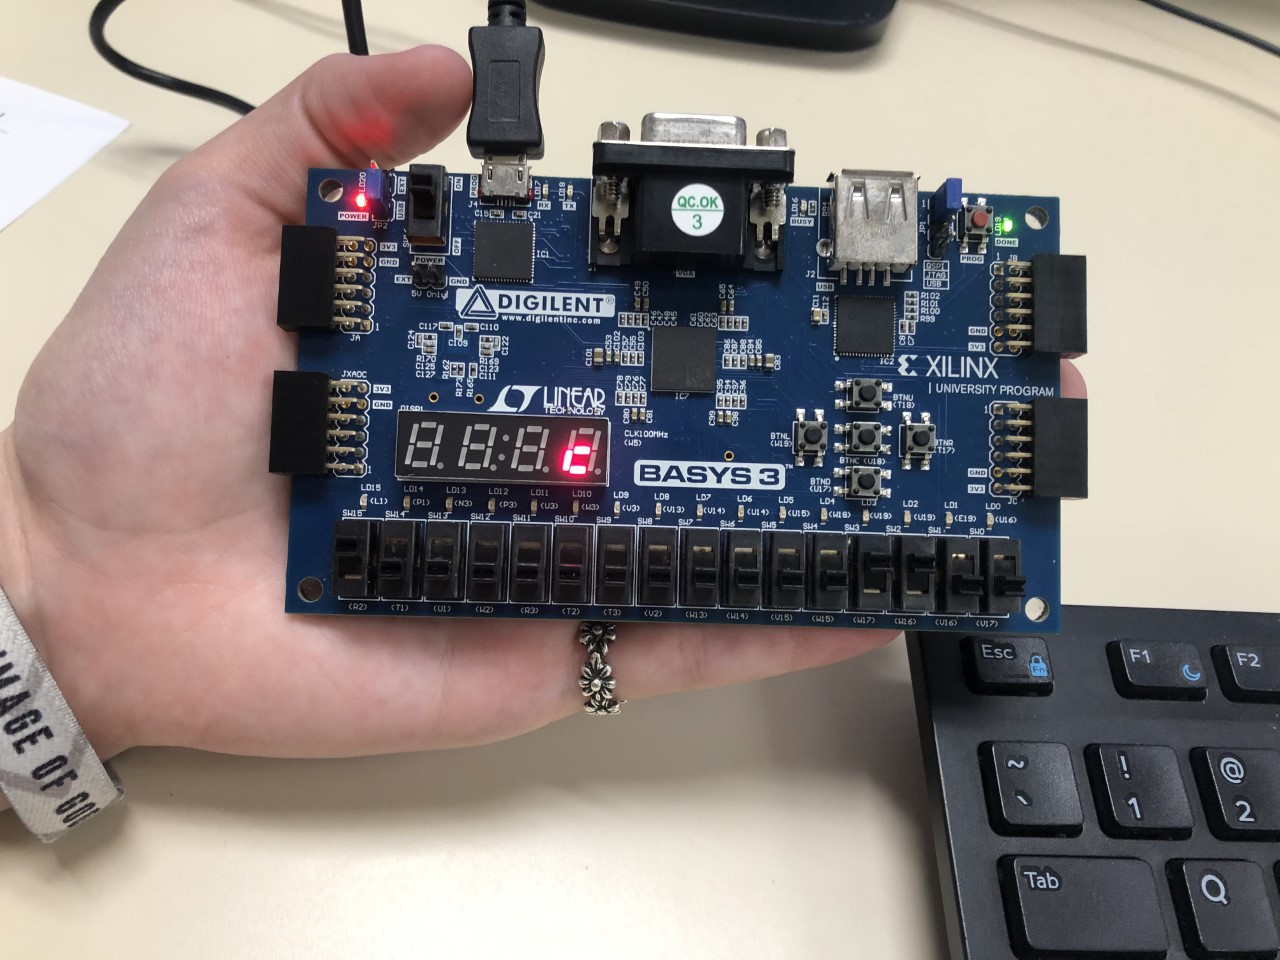
\includegraphics[width= 0.9\textwidth]{b1.png}
\caption{c displayed on first digit}
\label{fig: pic1}
\end{figure}

\begin{figure}[ht]\centering 
	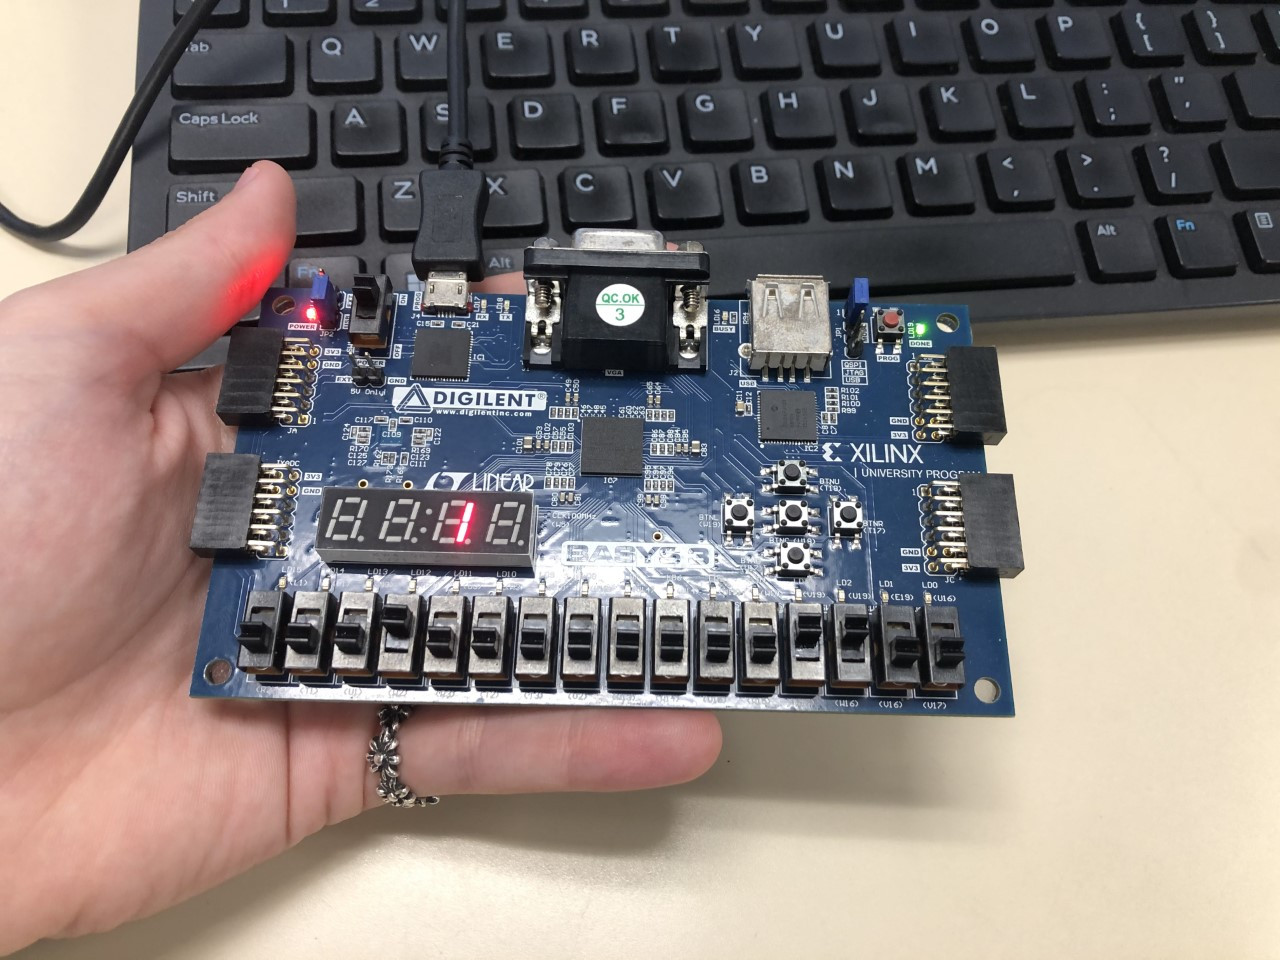
\includegraphics[width= 0.9\textwidth]{b2.png}
	\caption{1 displayed on second digit}
	\label{fig: pic2}
\end{figure}

\begin{figure}[ht]\centering 
	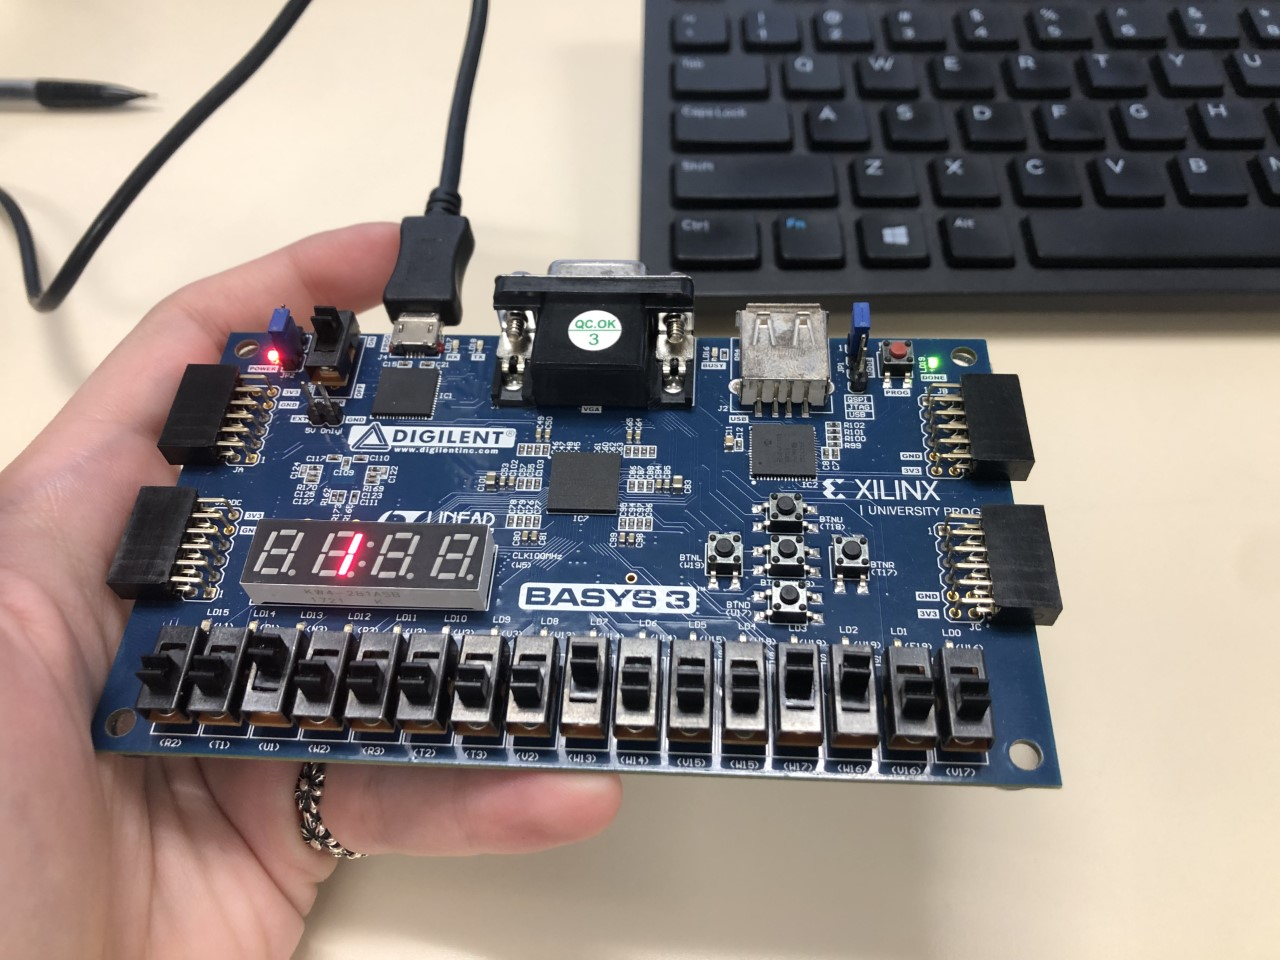
\includegraphics[width= 0.9\textwidth]{b3.png}
	\caption{1 displayed on third digit}
	\label{fig: pic3}
\end{figure}

\begin{figure}[ht]\centering 
	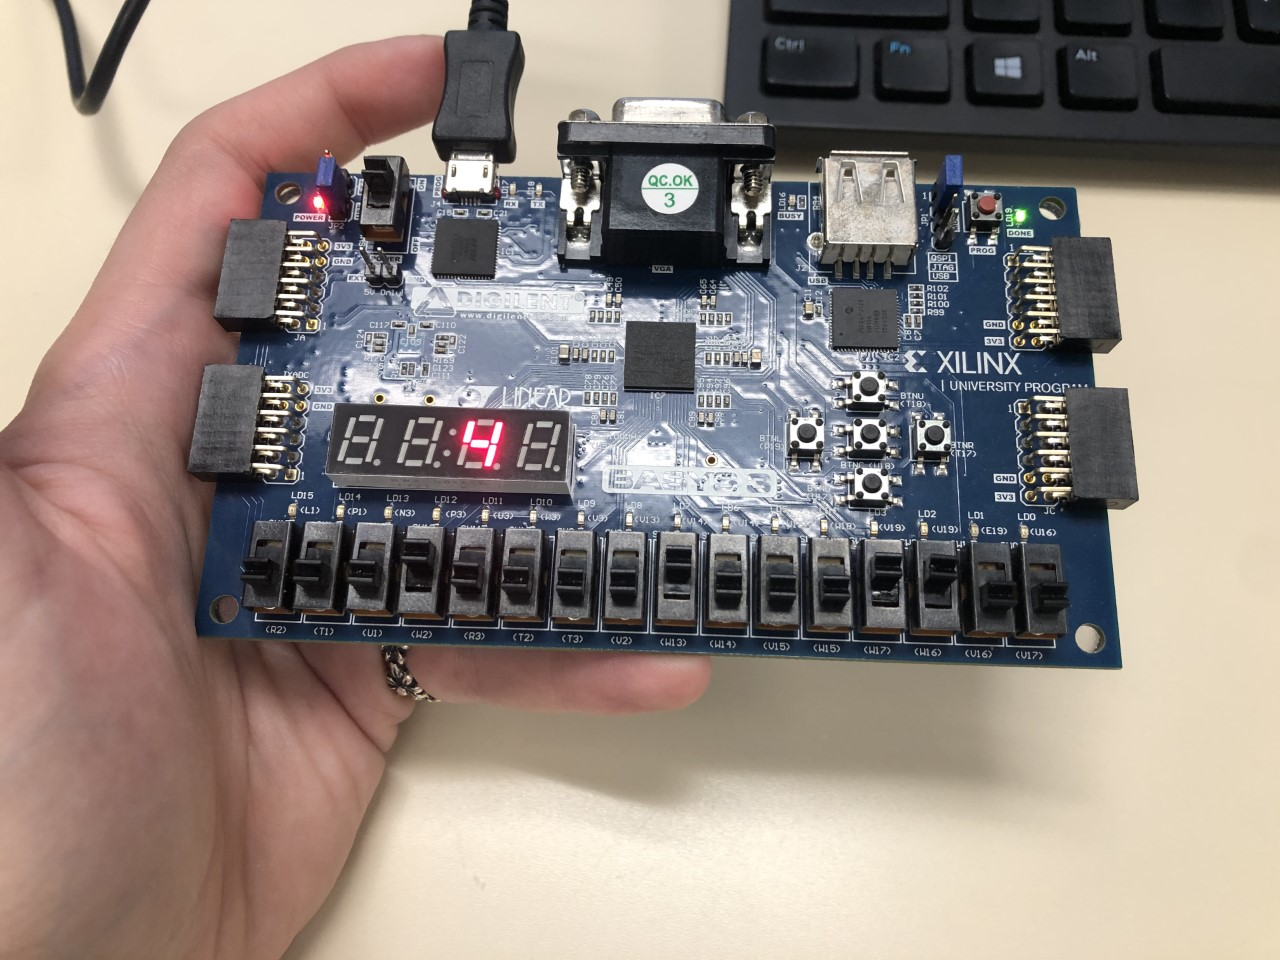
\includegraphics[width= 0.9\textwidth]{b4.png}
	\caption{4 displayed on second digit}
	\label{fig: pic4}
\end{figure}

\begin{figure}[ht]\centering 
	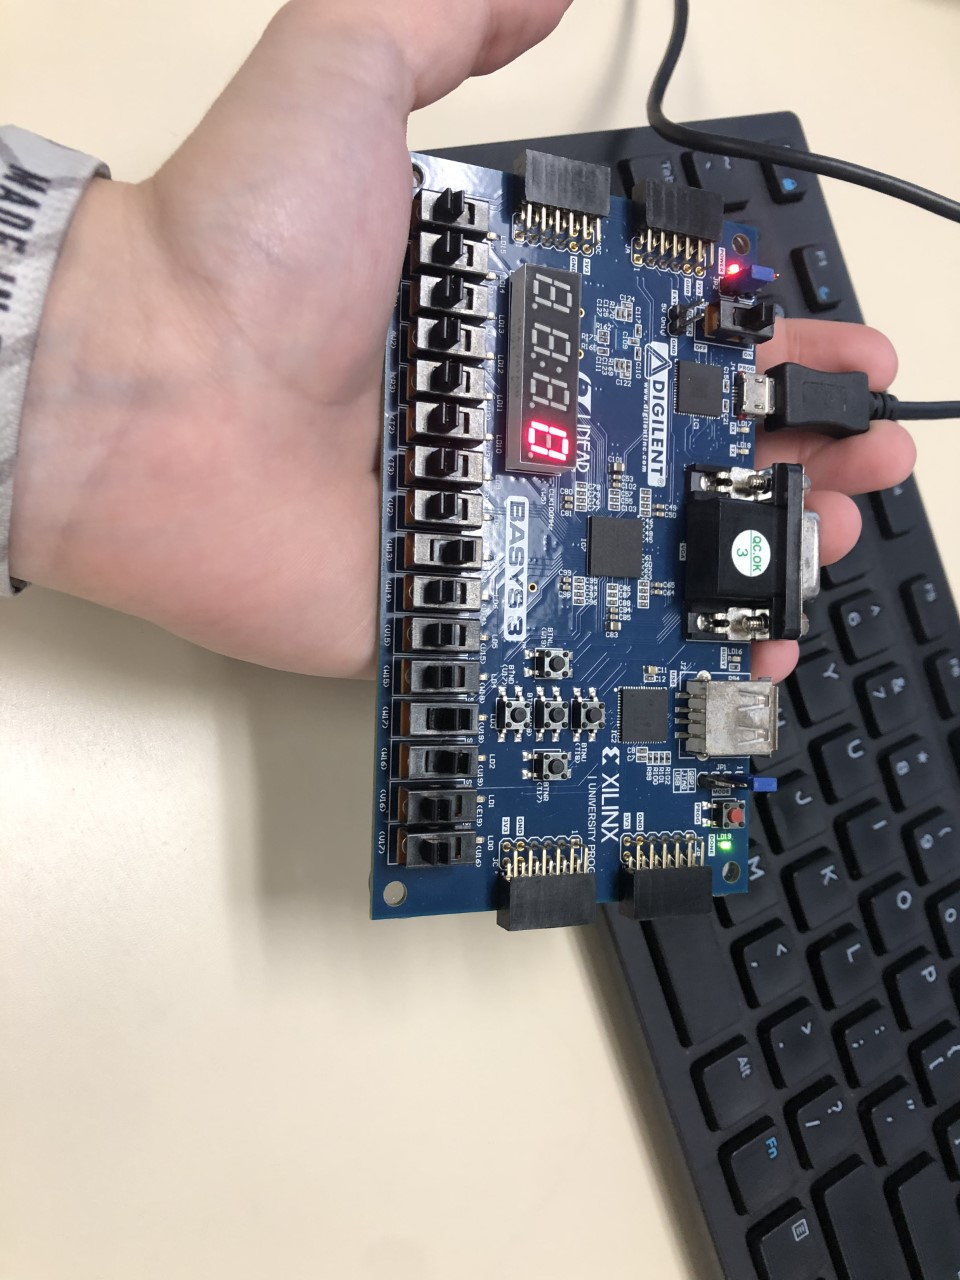
\includegraphics[width= 0.9\textwidth]{b5.png}
	\caption{0 displayed on first digit}
	\label{fig: pic5}
\end{figure}

\begin{figure}[ht]\centering 
	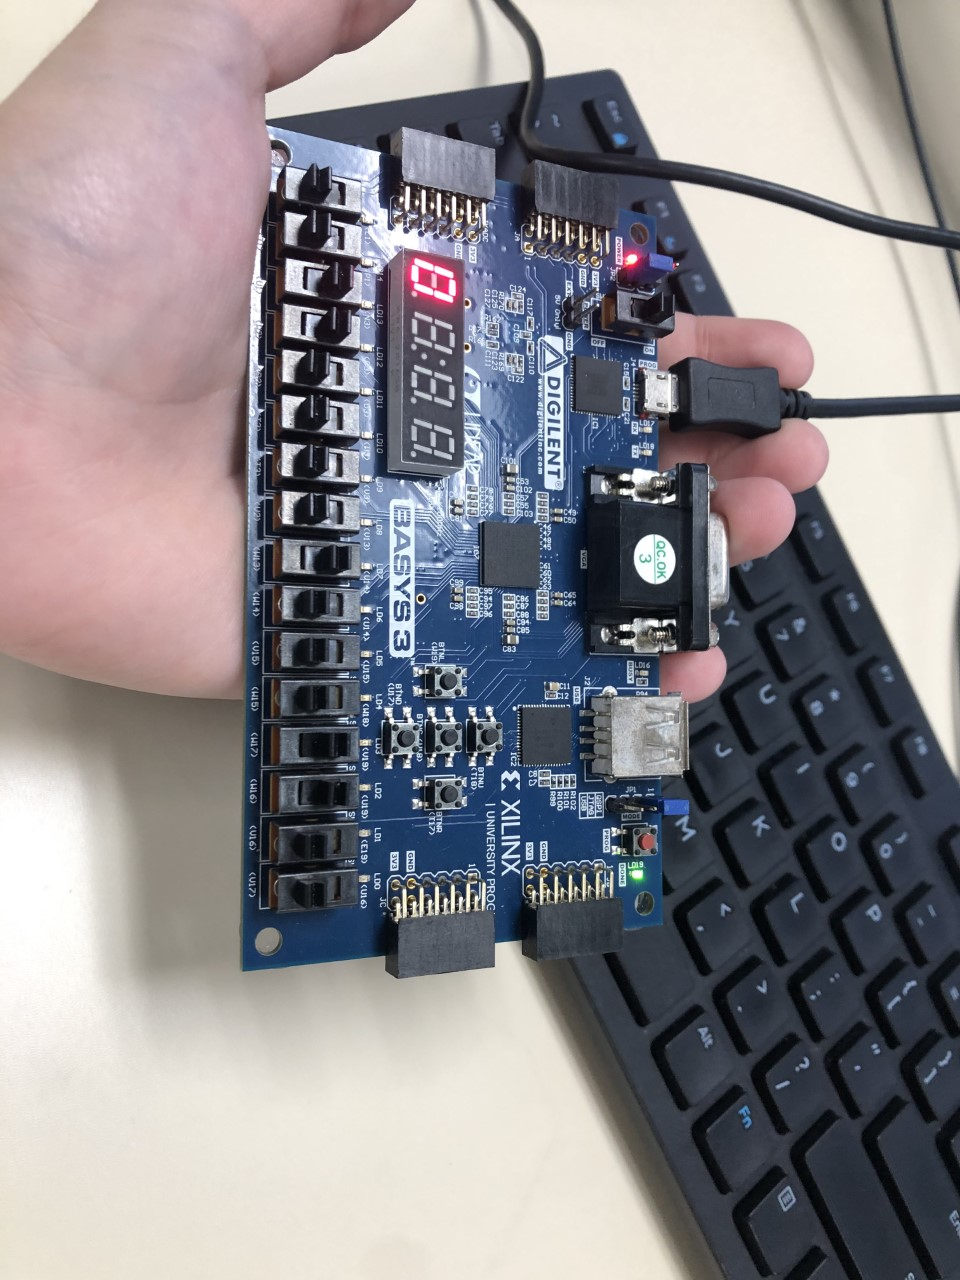
\includegraphics[width= 0.9\textwidth]{b6.png}
	\caption{0 displayed on fourth digit}
	\label{fig: pic6}
\end{figure}

\begin{figure}[ht]\centering 
	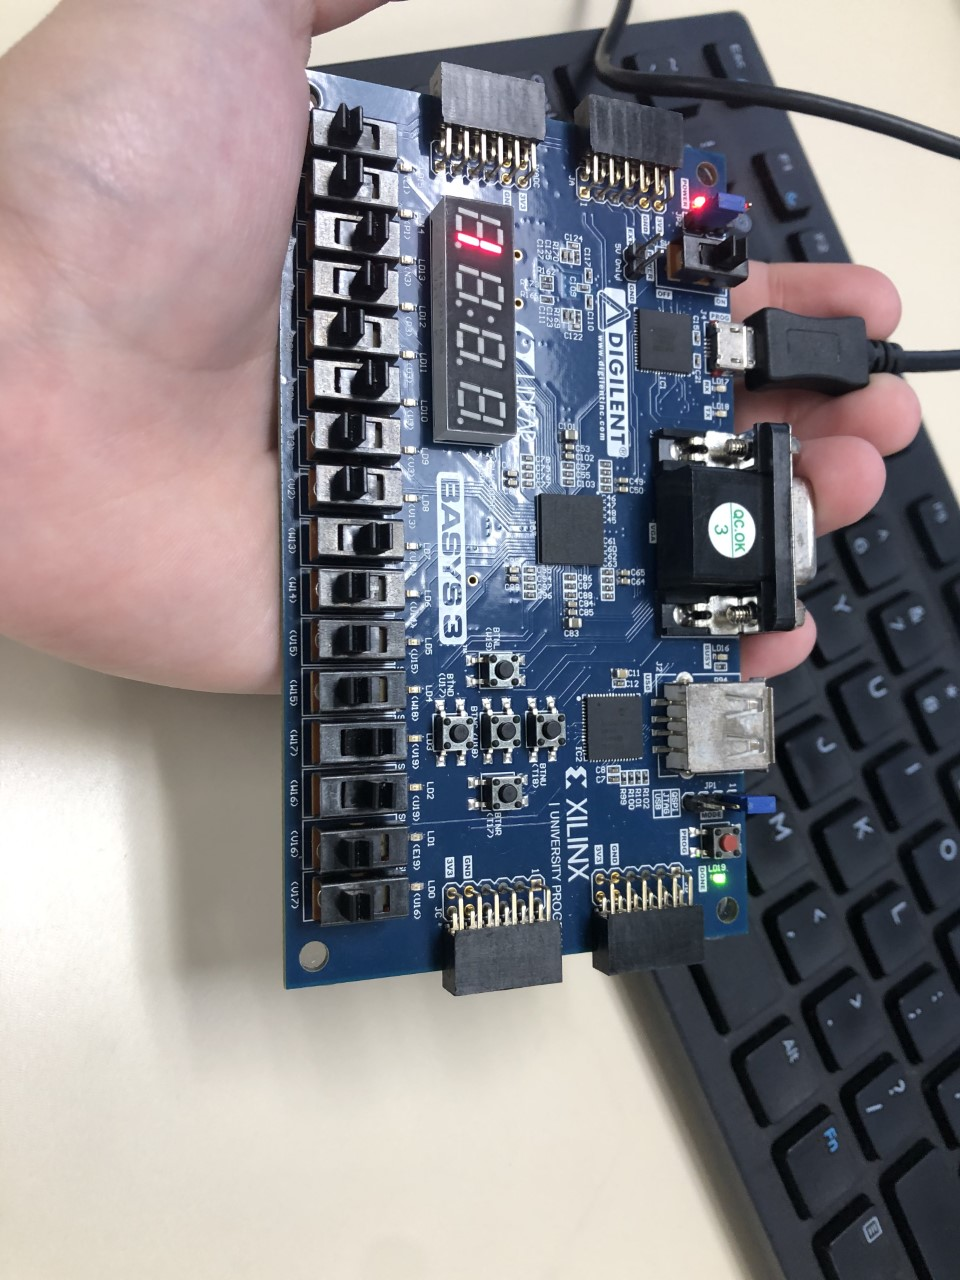
\includegraphics[width= 0.9\textwidth]{b8.png}
	\caption{1 displayed on fourth digit}
	\label{fig: pic7}
\end{figure}

\begin{figure}[ht]\centering 
	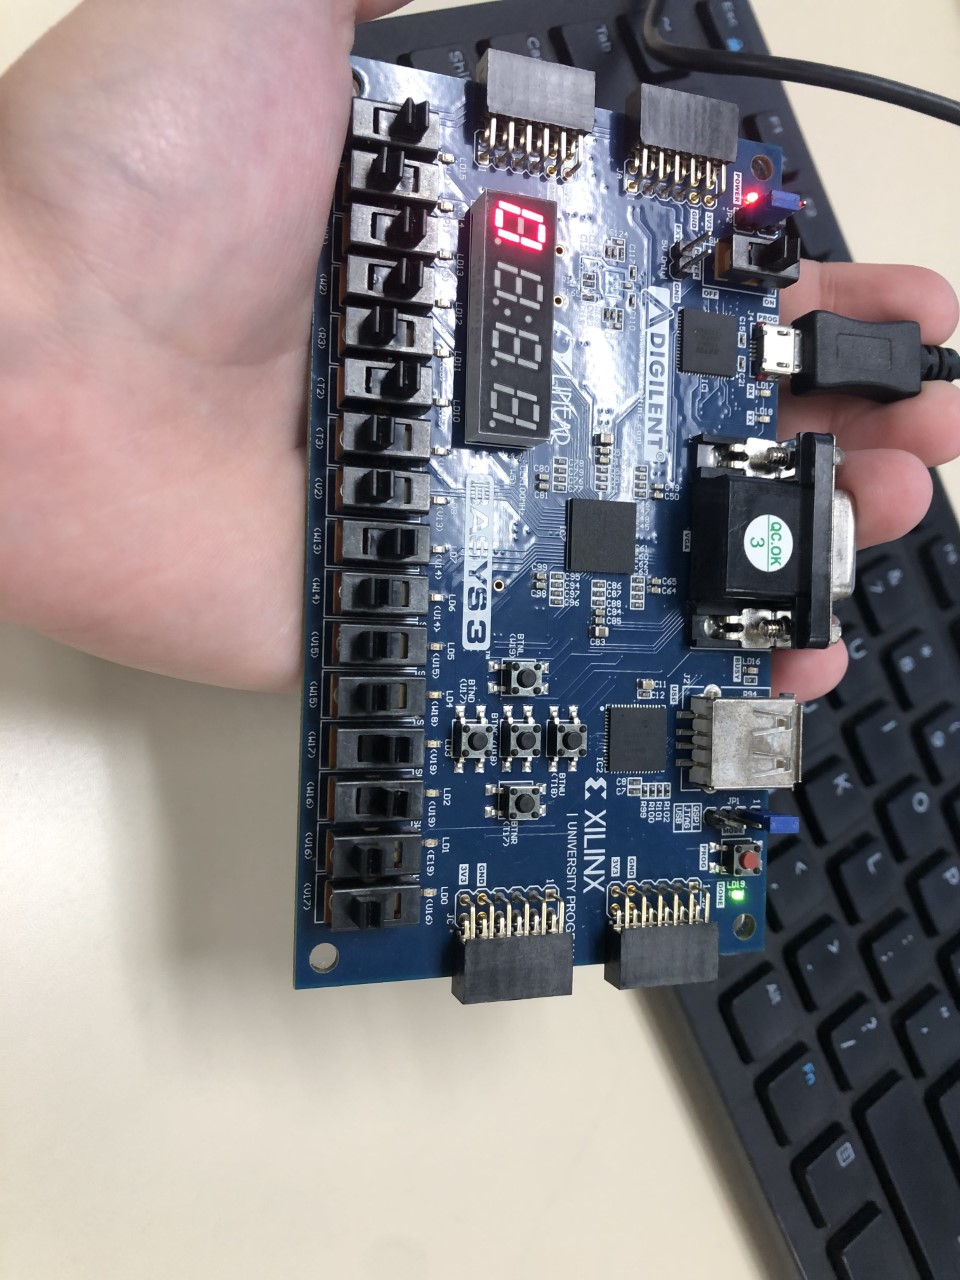
\includegraphics[width= 0.9\textwidth]{b9.png}
	\caption{0 displayed on fourth digit}
	\label{fig: pic8}
\end{figure}

\begin{figure}[ht]\centering 
	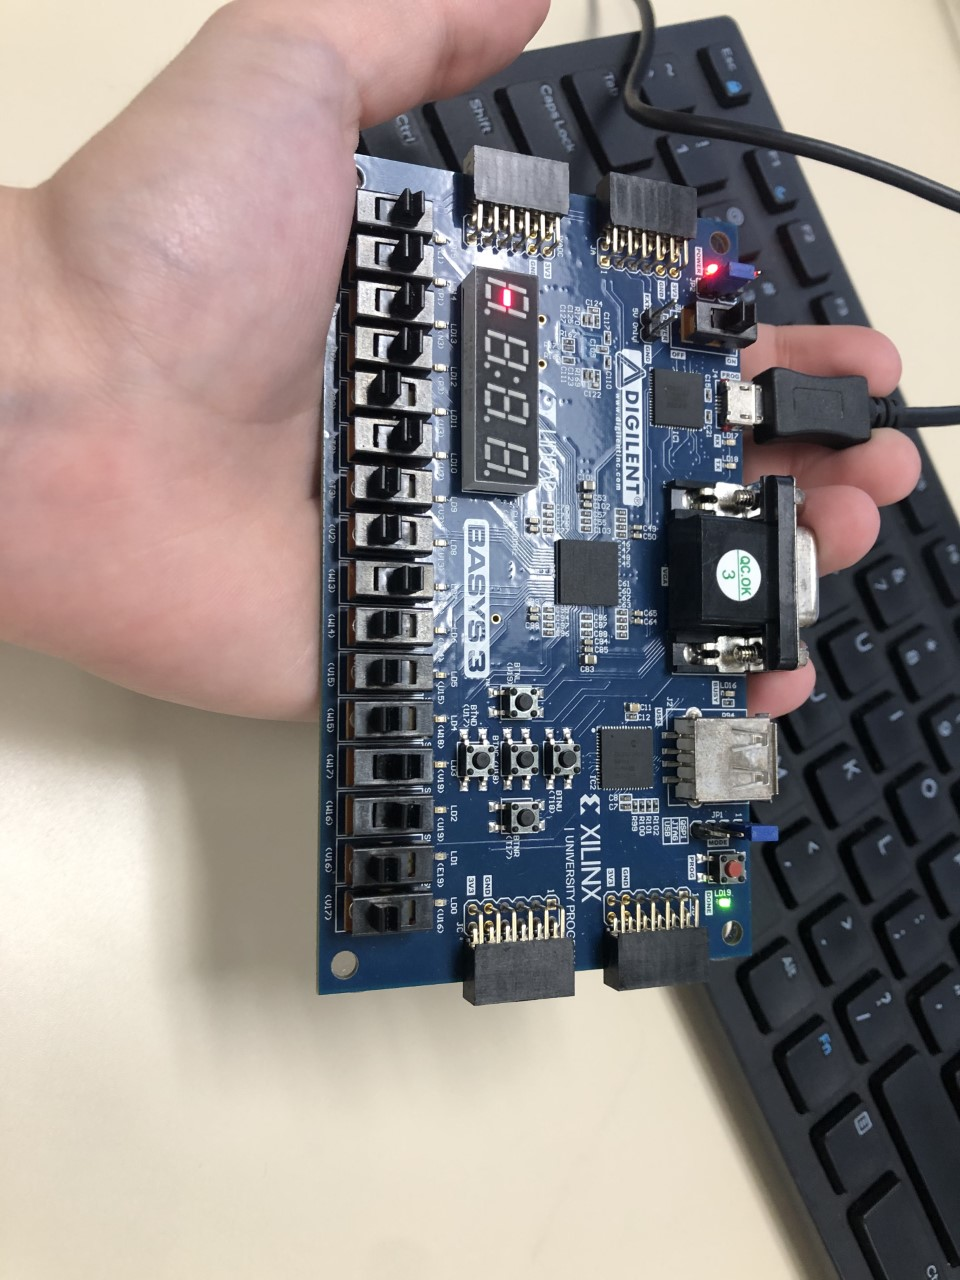
\includegraphics[width= 0.9\textwidth]{b10.png}
	\caption{- displayed on fourth digit}
	\label{fig: pic9}
\end{figure}

\begin{figure}[ht]\centering 
	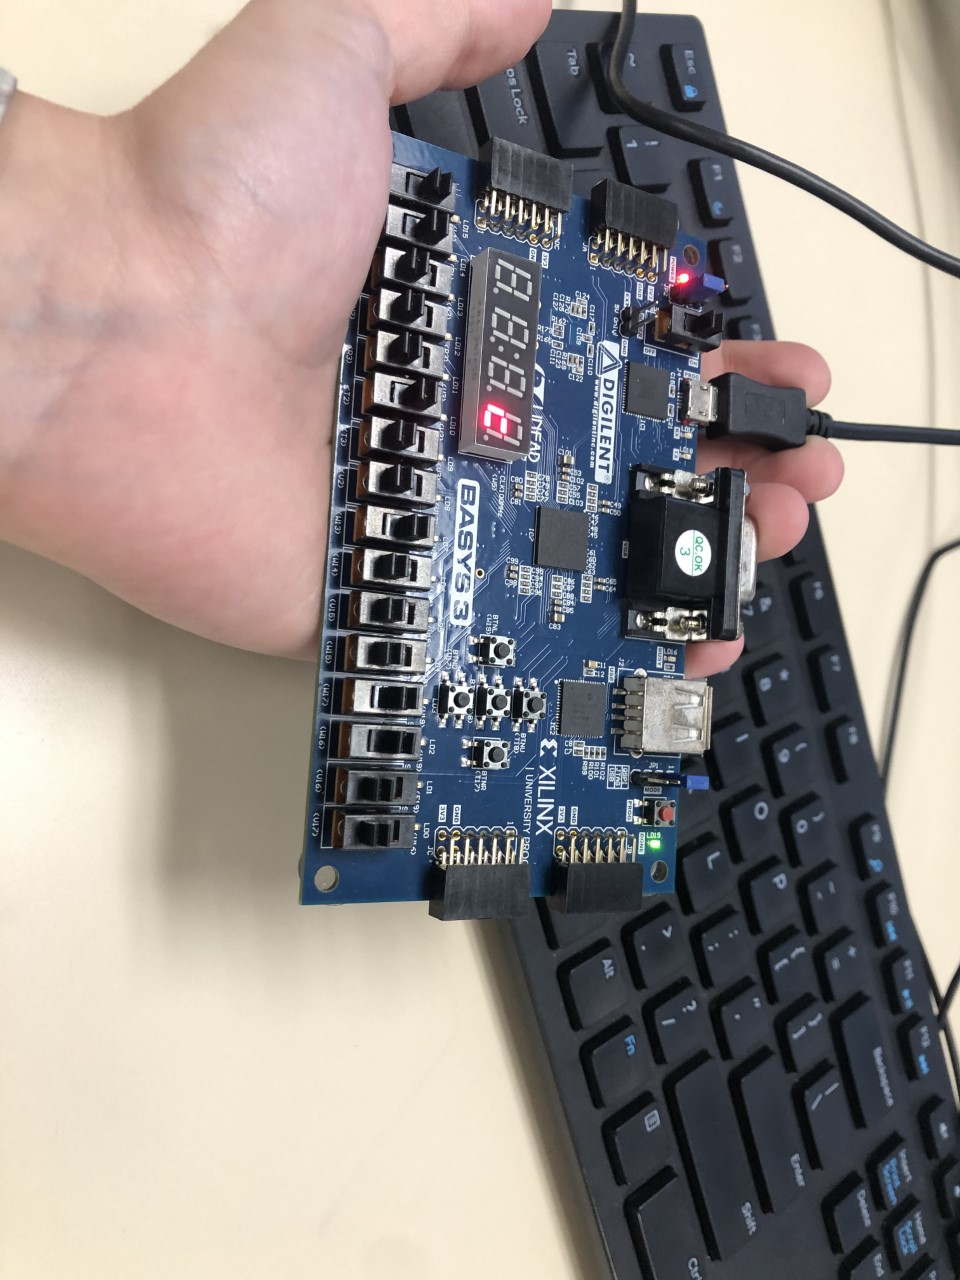
\includegraphics[width= 0.9\textwidth]{b11.png}
	\caption{c displayed on first digit}
	\label{fig: pic10}
\end{figure}

\begin{figure}[ht]\centering 
	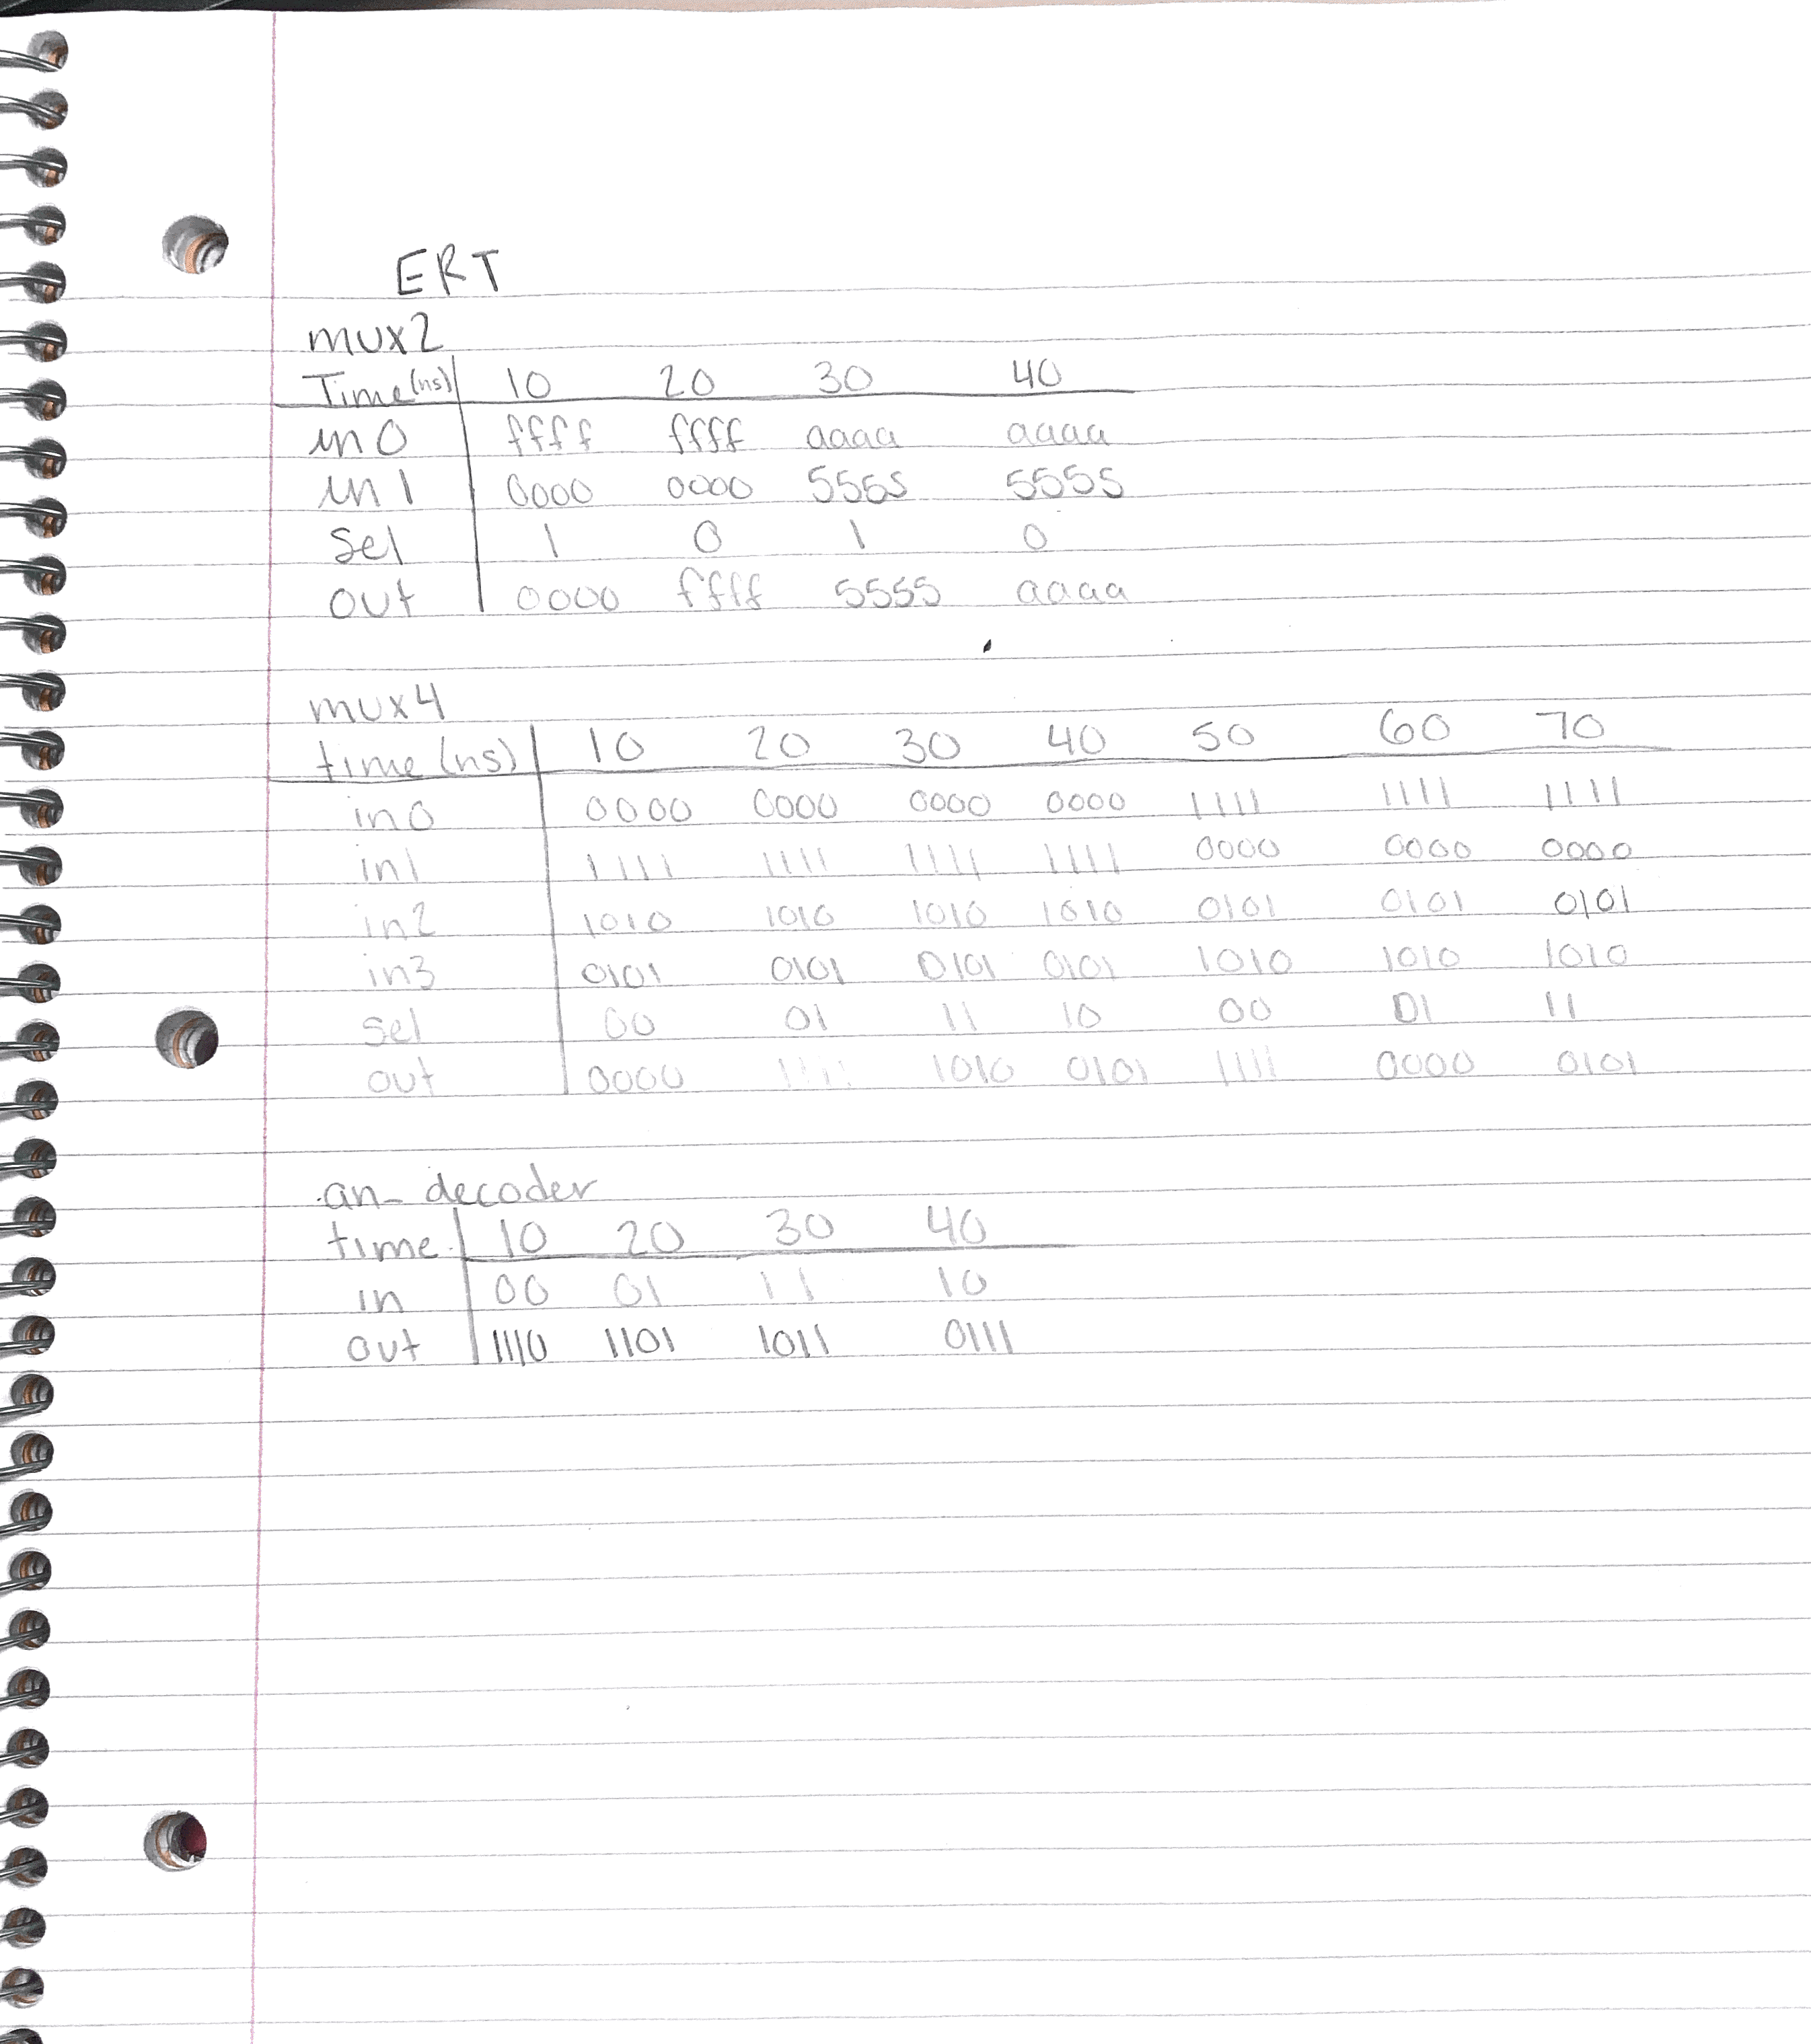
\includegraphics[width= 0.9\textwidth]{ert.png}
	\caption{ERTs}
	\label{fig: ert}
\end{figure}

\end{document}
